\begin{surferIntroPage}{Tutorial}{tutorial_koord1}{Primii pa\c si cu SURFER}
Acest program se nume\c ste SURFER. C\^and citi\c ti acest cuv\^ant v\u a g\^andi\c ti probabil la ap\u a,
soare \c si valuri. Totu\c si, \^\i n acest caz, numele provine din cuv\^antul englezesc {\it surface} (suprafa\c t\u a).
\\
Cu SURFER se pot reprezenta suprafe\c te, mai precis suprafe\c te algebrice. Ce \^\i nseamn\u a aceasta
\c si ce sunt suprafe\c tele algebrice este explicat \^\i n acest tutorial. Alege\c ti una din suprafe\c tele din partea dreapt\u a pentru a naviga prin capitolele acestui tutorial.\\
SURFER este parte integrant\u a a expozi\c tiei itinerante IMAGINARY care a \^\i nceput \^\i n 2008 care a
fost declarat Anul Matematicii \^\i n Germania. Expozi\c tia este un proiect al binecunoscutului Institut
de Cercet\u ari Matematice de la Oberwolfach situat \^\i n Mun\c tii P\u adurea Neagr\u a din Germania. Aici au loc \^\i n fiecare s\u apt\u am\^an\u a conferin\c te pe teme recente din cercetarea matematic\u a. Aceste conferin\c te sunt importante pentru a impulsiona schimburile academice \^\i n jurul globului. \\
\vspace{0.2cm} \hspace{3.5cm}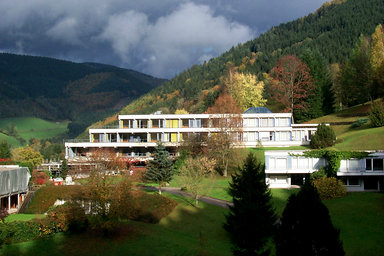
\includegraphics[width=3cm]{./../../common/images/photo_mfo.jpg}\\
Programul SURFER poate fi desc\u arcat gratuit de pe pagina noastr\u a: \\
\begin{centering}
www.imaginary.org\\
\end{centering}
 \vspace{0.2cm}
\^In partea dreapt\u a pute\c ti alege unul dintre tutorialele matematice \^\i ncep\^and cu suprafa\c ta Citric\u a. \^In partea st\^ang\u a pute\c ti merge la alte galerii, de exemplu la galeria despre suprafe\c te fantastice.
\end{surferIntroPage}